\chapter{Experiment}
In the previous chapter we described the design details that we will be using to implement the experiment. In this Chapter we go into the implementation details of the project.

\section{Infrastructure setup}
We will start of by first setting up the virtual network with the OVS Switches running the traditional MPLS System. To do this we first set up the mininet virtual network with the OpenVSwitch switches and hosts as described in Figure 2.5. Once the network system is in place we add the MPLS flows to the switches using OpenFlow. And finally we run a ping test to pass the ICMP packets through the MPLS switches to test the system.

\subsection{Setting up Mininet and OpenVSwitch}
The Mininet tool package is available in the Advanced Package Tool (APT) of all Linux Distributions. It can be easily installed on the system using the package name 'mn'. The Mininet package has a dependency on OVS packages and thus are installed along with the mininet package by the APT command.\\
\\
The Network topology can be set up by calling the command:\\
\\
\textit{sudo mn --topo=linear,3 --switch=ovsk --controller=ovsc}\\
\\
The parameter meanings are as follows:
\begin{enumerate}
\item --topo=linear,3 \\
This parameter creates a topology of 3 switches each with their own host connected in a linear fashion.
\item --switch=ovsk \\
This parameter determines the type of switch that will be created in the mininet network. The value 'ovsk' indicates that OVS switches that run in kernel space are to be created
\item --controller=ovsc \\
This parameter determines the type of controller that will be created in the mininet network. this controller is responsible for forwarding the flow rules and actions to all the switches in the network. the value 'ovsc' indicates that an OVS controller is to be created to communicate with the OVS switches.
\end{enumerate}


\section{Testing the MPLS System}
\subsection{Addition of the MPLS flows}
Once the network infrastructure is set up we then add the MPLS Flows to the switches via the OVS controller. This is done passing the flow rules and actions to the Openflow Switch Manager (ovs-ofctl).\\
\\
The OpenFlow Switch management command structure is as follows: \\
\\
\textit{ovs-ofctl -O OpenFlow13 add-flow s1 "table=0,in\_port=1,eth\_type=0x800,actions=goto\_table:1}"
\\
\begin{enumerate}
\item -O OpenFlow13\\
Indicates the OpenFlow Version to use. The value 'OpenFlow13' indicates OpenFlow Version 1.3.
\item add-flow s1\\
Indicates the action to be taken on the switches. We can add flows, delete flows modify flows etc using the OpenFlow Protocol. The value 's1' indicates the switch on which the flow rules are to be added.
\item "table=0,in\_port=1,eth\_type=0x800,actions=goto\_table:1" \\
Is the flow rule where the flow is to be added in table '0' of the Switch, to packets arriving at port '1' which is mapped to interface s1-eth1, which are of eth type 0x800 (ICMP Packets). The 'actions' value indicates the type of actions to take on such packets.
\end{enumerate}

The Complete Flow configuration for MPLS is as follows:

\begin{figure}[H]
       \centering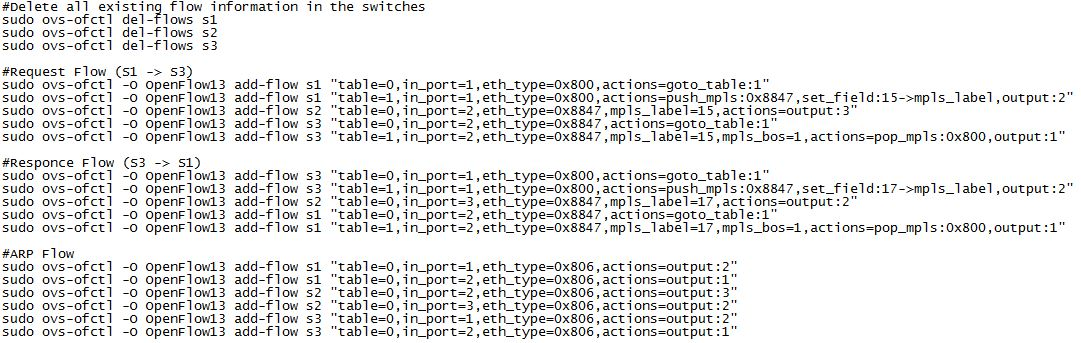
\includegraphics[width=\textwidth]{images/10_Open_Flow_flows_for_MPLS.JPG}
       \caption{OpenFlow Flow Scripts for traditional MPLS}
       \label{fig:compbest}
\end{figure}

\subsection{Testing Communication for MPLS}
After adding the Flow Rules we can initiate the ping test from h1 to h3 by calling the ping command in the Mininet CLI. This would create an ICMP packet at Host H1 which would be forwarded to Switch S1. Switch S1 based on the Flow Rules as described in Figure 3.1 will forward the packet to its table '1' where it will push an MPLS label of eth value 0x8847, set its label value to 15 and forward it to switch S2. Switch S2 will redirect all packets of eth type 0x8847 and MPLS Label value 15 to Switch S3. S3 based on its flow rules will first forward the data packet to its table 1 where it will check if the MPLS label has value 15 and is a bottom of the stack label, pop the MPLS label if it is and later forward the packet to Host H3. H3 then responds to the ICMP request by sending the ICMP response to switch S3 after which the data packets is subjected to the flow rules as described in the 'Response Flow' part of the diagram.

To test if the packets are being routed correctly using MPLS labels we can inspect the packets at switch 2. This is done by calling the command 'tcpdump' on one of the interfaces of switch 2. Refer diagram

\begin{figure}[H]
       \centering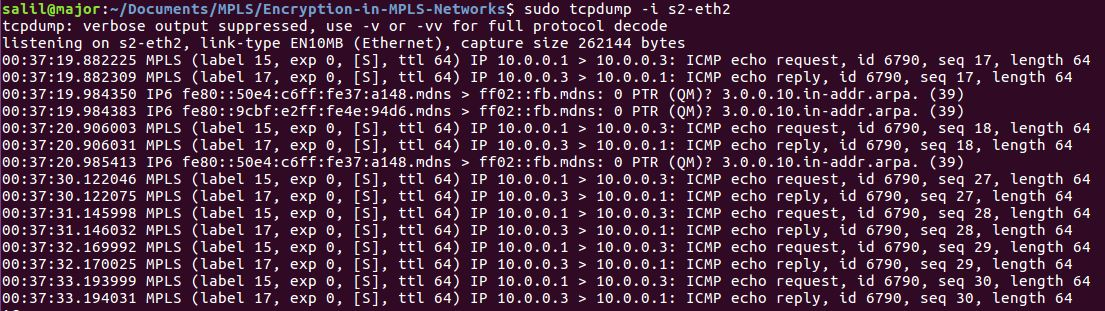
\includegraphics[width=\textwidth]{images/11_TCP_Dump_Capture_for_MPLS.JPG}
       \caption{'tcpdump' response for MPLS network traffic}
       \label{fig:compbest}
\end{figure}

The output displayed by the ping command in diagram indicates that the switches are pushing, inspecting and popping the MPLS labels correctly without any issues as shown in Figure 3.3.

\begin{figure}[H]
       \centering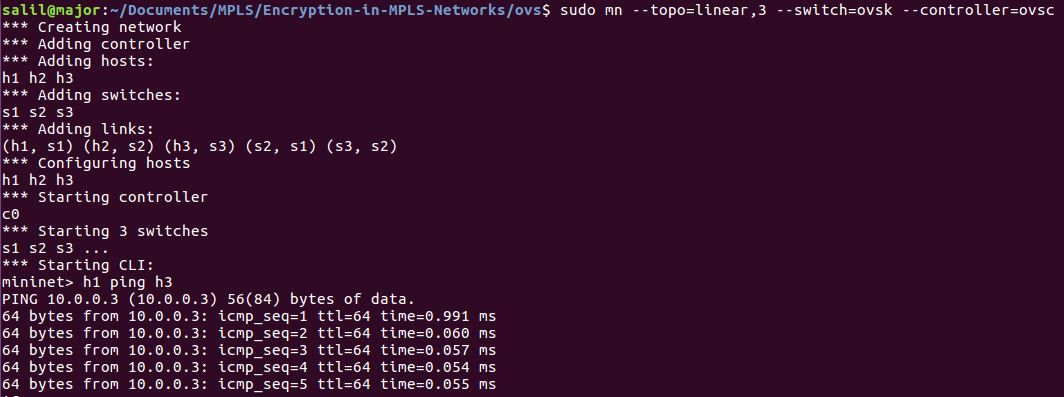
\includegraphics[width=\textwidth]{images/12_ICMP_responce_for_MPLS.JPG}
       \caption{'ping' response for MPLS Network Traffic}
       \label{fig:compbest}
\end{figure}


\section{Implementation of OS Encryption functionality}
The next part of the experiment involves the implementation of the OS Encryption functionality. Based on the OS designed as mentioned in chapter 2, the four additional functionality involved in the MPLS OS is the addition and removal of the CW and the Encryption and Decryption of the MPLS Payload. These functionalities should be performed by the OVS Switch involved in the network experiment and as such should be implemented in the OVS code base. 

After a thorough study of the OpenVSwitch codebase, we found out that there is no such inbuilt provision in the OVS codebase for the required Os functionality. We can neither implement the CW functionality nor the Encryption/Decryption of the MPLS payload with the currently existing features of OVS. The functionality was thus needed to be implemented manually into the OVS codebase and then converted into a kernel module for the Switches to implement the same at the kernel level.

For the sake of development classification we will segregate the OS functionality into 2 categories:

\subsection{Changes at the Ingress (Entering) Switch}
When the ICMP request packet from H1 enters S1, before pushing the MPLS header on the data packet, S1 first encrypts the payload data using AES-GCM encryption algorithm. The key and IV required for the encryption is currently hardcoded in the code as their values are dependent on the Key Exchange which is not implemented in this project. The AEAD-AES-GCM encryption is carried out using the Linux Kernel Crypto API\footnote{Kernel Crypto API is a cryptographic framework in the Linux Kernel for various kernel implementations dealing with cryptography}. After encryption the pseudo wire CW is pushed on top of the encrypted data followed by pushing the MEL on top of it.

Due to certain implementation aspects of the Linux Kernel Crypto AEAD encryption API, instead of encrypting the Payload data first and then adding the CW we will first add the CW and then encrypt the underlying Payload. The details of this aspect will be discussed further in this section.

\subsubsection{Insertion of CW}
We first create the CW data structure in the OVS codebase and assign the nonce value to the CW sequence attribute. 

%insert CW structure

In OVS datapath and Linux kernel in general, all data packets are parsed into a fundamental data structure called a socket buffer (skb)\footnote{The socket buffer, or "SKB", is the most fundamental data structure in the Linux networking code. Every packet sent or received is handled using this data structure.}. The skb is a series of contiguous memory location storing the data packet information in the form of bytes. The structure of the skb is shown in Figure 3.4.

\begin{figure}[H]
       \centering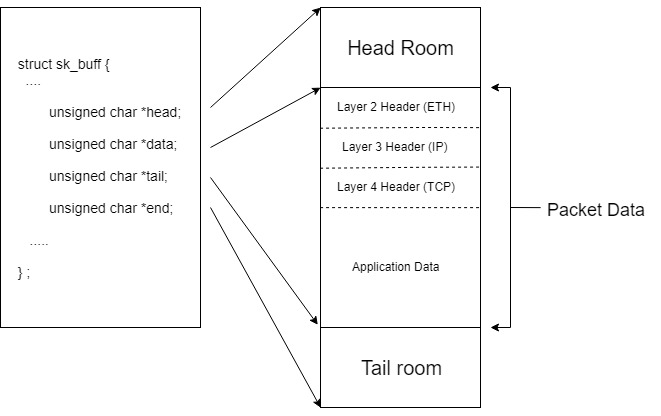
\includegraphics[width=\textwidth]{images/13_SKB_Data_Structure.jpg}
       \caption{SKB Data Structure}
       \label{fig:compbest}
\end{figure}

Any changes that involve manipulating the data packet have to be done by manipulating the data bits of the skb data structure. A number of data pointers help map the various data and header locations in the skb structure. The linux kernel has in-built APIs to manipulate these contents. It is highly recommended to use these API's as the various pointer in the skb data structure are heavily interdependent on each other. Using these APIs we manipulate the data packet and insert our CW between the payload and the MAC header of the datapacket. This is done by calling the following series of Kernel APIs. Refer Table 3.1 which depicts the implementation of the skb kernel APIs to insert the CW into the data packet.\\

\begin{table}[H]
\centering
\begin{tabular} { | m {0.9cm} | m {5cm} | m {8cm} | }
\hline
Sr.no & Command & Function \\
\hline
\hline
 1 & skb\_cow\_head & Checks if space, the size of the CW header, is available in the headroom for inserting the CW. \\ 
 \hline
 2 & skb\_push & Allocates the space for the Data Structure. \\ 
 \hline
 3 & memmove & Moves the MAC header to the newly allocated space so that the CW can be inserted between the MAC header and the underlying payload. \\
 \hline
 4 & skb\_reset\_mac\_header & Resets the MAC header pointer to the new MAC header position.  \\
 \hline
 5 & skb\_mac\_header(skb) + skb->mac\_len & Points to the start of the CW memory space where the CW data bits can be filled. \\
\hline
\end{tabular}
\caption{Steps to insert CW in Data packet}
\label{table:1}
\end{table}

\subsubsection{Encryption of Data using Linux Crypto API}
The Linux Kernel Crypto API is a rich set of cryptographic ciphers and data transformation API used for cryptographic operations at the kernel level. To understand and properly use the Crypto API functions one needs to understand their underlying architecture specifications and the functional flow of these APIs.

The Kernel Crypto API refers to all encryption algorithms as 'transformations'. The encryption is carried out by 2 major components, The transformation object, also called 'Cipher Handles' and the request handle. The transformation object contains all the settings and configurations of the given encryption type to use. The request handler as the name suggest handles the encryption request.

\begin{table}[H]
\centering
\begin{tabular} { | m {0.9cm} | m {5cm} | m {8cm} | }
\hline
Sr.no & Command & Function \\
\hline
\hline
 1 & Initialize 'crypto\_aead' and 'aead\_request' & Initialize the AEAD transformation Object and its Request Handler \\ 
 \hline
 2 & crypto\_alloc\_aead & Allocate the AEAD Cipher Handle\\ 
 \hline
 3 & aead\_request\_alloc & Allocate the AEAD Request Handle \\
 \hline
 4 & aead\_request\_set\_callback & Set the Asynchronous callback function that will be executed once the encryption is successfully completed \\
 \hline
 5 & crypto\_aead\_setkey & Set the encryption key in the cipher handle \\
  \hline
 6 & aead\_request\_set\_crypt & Set the data buffers where the encryption process will happen. The data that is to be encrypted is concatenated with the allocated data at the start and then passed as whole as plain text \\
 \hline
 7 & aead\_request\_set\_ad & Set the associated data information that will be used to generate the authentication tag for authentication of data at the receiving end \\
 \hline
 8 & crypto\_aead\_encrypt & Start the encryption process\\
\hline
\end{tabular}
\caption{Steps to Encrypt the Data Payload}
\label{table:1}
\end{table}

Table 3.2 describes the flow of API calls to initiate the encryption of the packet data.

Once the payload data has been encrypted S1 can then further push the MEL label on top of the packet followed by the Special Purpose Label Packet and another normal MPLS packet for routing.

\subsection{Changes at the Egress (Exiting) Switch}
Once the encrypted MPLS OS packet reaches the Egress Switch S3, S3 pops the top MPLS label along with the MEL. It then inspects nonce value in the CW header. If the nonce counter value matches with the counter value of switch S3 then the switch moves ahead with the decryption. 

\subsubsection{Decryption of Data using Linux Crypto API}
Decryption of the MPLS payload follows the same procedure as the one during Encryption process with a slight change in the input values to the API's. During decryption, the cipher text is passed in the place of plain text into the API's. The cipher text is a concatenated combination of the associated data, ciphertext and authentication tag. Also in the crypto\_aead\_encrypt function the flag is set to decrypt. The decryption process authenticates the packet using the authentication tag. The process can send out an alert if the authentication tag fails to authenticate. The output of the decryption gives us a concatenated combination of the associated data and the plain text. 

\subsubsection{Removal of CW}
Just as how we used the in-built SKB manipulation APIs to insert the CW in the Ingress Switch, we will use the same approach while removing the CW from the Data packet. Refer Table 3.3 which depicts the implementation of the skb kernel APIs to remove the CW from the data packet.

\begin{table}[H]
\centering
\begin{tabular} { | m {0.9cm} | m {5cm} | m {8cm} | }
\hline
Sr.no & Command & Function \\
\hline
\hline
 1 & skb\_postpull\_rcsum & Recalculate the checksum after pulling the MEL from the data packet\\ 
 \hline
 2 & memmove & Moves the MAC header to occupy the place where the CW resides \\ 
 \hline
 3 & \_\_skb\_pull & Pulls the CW size equivalent of data from the top of the data structure which was redundant as the MAC header shifted down.  \\
 \hline
 4 & skb\_reset\_mac\_header & Resets the MAC header pointer to the new MAC header position.  \\
 \hline
 5 & skb\_set\_network\_header & Sets the network header pointer to the new network header position. \\
\hline
\end{tabular}
\caption{Steps to remove the CW from the Data packet}
\label{table:1}
\end{table}


\section{Testing the MPLS OS System}
Once the OS functionality has been implemented in the OVS code-base we need to deploy it into out experimental system for testing. This is done by first building the code base to create its binaries. The OVS code has a Make files that has all the file building sequences scripted into it. Using the Linux 'make' command you can compile the system. Once the System has compiled successfully you call the Linux function 'make install' to install all the binaries into the appropriate locations in the system. We then remove the currently loaded OVS module by calling 'rmmod openvswitch' function so we can load the new module containing the MPLS OS functionality. We then run the 'make modules\_ install' function to build the kernel module libraries and install them the the Kernel modules directory. Finally we load the newly installed openvswitch kernel module by calling 'modprobe openvswitch'.

\subsection{Addition of the MPLS OS flows}
The MPLS Flows for OS are similar to the ones mentioned for traditional MPLS. The only difference being the addition of the Special Purpose Label with value 15, the MEL and the CW. However the addition of these headers is not a part of the OpenFlow Flow. The addition of these headers depends on the success of Key Exchange between the Ingress and Egress LSR's before the OS can begin and thus the LSRs must be programmed to take that decision programmatically. Since we are not implementing the Key exchange in this experiment and have hard coded the key for experimental purposes. We are allowed to instruct the LSRs to force push the MEL of value 1 followed by the Special purpose MPLS Label with value 15 and another MPLS Label for routing purposes. Addition of CW is programmed internally in the OS functionality.
	During Experimentation however, it was observed that the Egress switch would drop these packets. The MPLS OS packets would route through switch S2 but S3 would drop these packets before forwarding to Host H3. Analysis into the issue led to the discovery of issues in OVS with respect to contiguous popping off of 2 or more Labels (MPLS and even VLAN). It was observed that at the kernel level OVS is only able to push and pop one Label. 2 or more contiguous labeled packets are routed to the Userspace for efficient handling. However for some reason the Userspace fails to do so. This issue is apparently prevalent in OVS and concerns were been raised back in 2016. However no information was found regarding its solution. More details can be found in this mailing list \cite{OVSmail1} \cite{OVSMail2}
    As a result a work-around was implemented which would not affect the overall aim of the project. Instead of pushing the MEL, the special purpose MPLS label with value 15 and the normal MPLS Label, we decided to push just one MPLS Label of label value 1. This Label will act as a functional combination of all the 3 labels in our experiment and would not interfere with the OS Encryption as a whole.
    So based on this work-around the Flow configuration for MPLS with OS is as follows:
    
\begin{figure}[H]
   \centering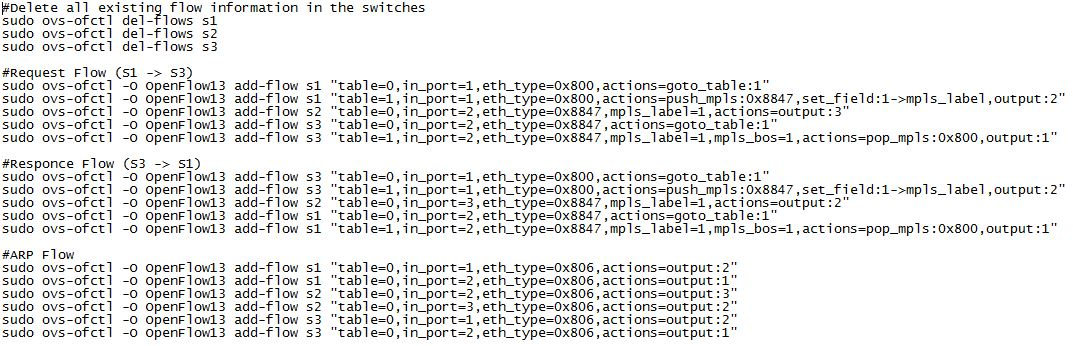
\includegraphics[width=\textwidth]{images/14_Open_Flow_flows_for_MPLS_OS.JPG}
   \caption{OpenFlow Flow Scripts for MPLS with OS}
    \label{fig:compbest}
\end{figure}

\subsection{Testing Communication for MPLS with OS}
The behavior of the MPLS System with the OS is similar to the behavior without the OS. The only difference to note is that in the MPLS OS Switch S1 will be encrypting the data packet and inserting the CW along with the MPLS Label with value 1 before forwarding it to Switch S2. S2 must not be able to sniff the internal data of the encrypted packet and must be able to forward it only based on the MPLS Label value. Once the MPLS OS packet reaches Switch S3, S3 should decrypt the packet, remove the CW and pop the MPLS Label before forwarding the original ICMP packet to host H3. Host H3 will respond to the packet with the response ICMP packet which follows the reverse path with encryption on S3 and decryption on S1.

To test if the packets are being encrypted correctly using the MPLS OS, we can inspect the packets at one of S2's interface. This is done by calling the command 'tcpdump' on one of the interfaces of switch 2. Refer diagram

\begin{figure}[H]
   \centering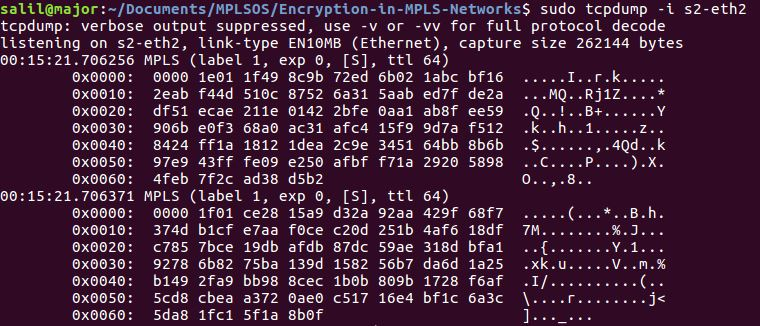
\includegraphics[width=\textwidth]{images/15_TCP_Dump_Capture_for_OS.JPG}
   \caption{'tcpdump' response for MPLS OS}
    \label{fig:compbest}
\end{figure}

As we can see in Figure 3.6 tcpdump tries to sniff the contents of the data packets and is unable to interpret its contents. The only understandable part being the MPLS header with value 1. The rest of the contents is dumped as it is in hexadecimal byte form. S2 cannot interpret that the contents of the IP packet are infact ICMP as we saw during the communication testing of traditional MPLS system in section 3.2.2.

The output displayed by the ping command in Figure 3.7 displays the proper response being received for each ICMP request packet. This means that the receiving switch is able to correctly decrypt the packet at its end and get the original ICMP packet as was sent by the sender.

\begin{figure}[H]
   \centering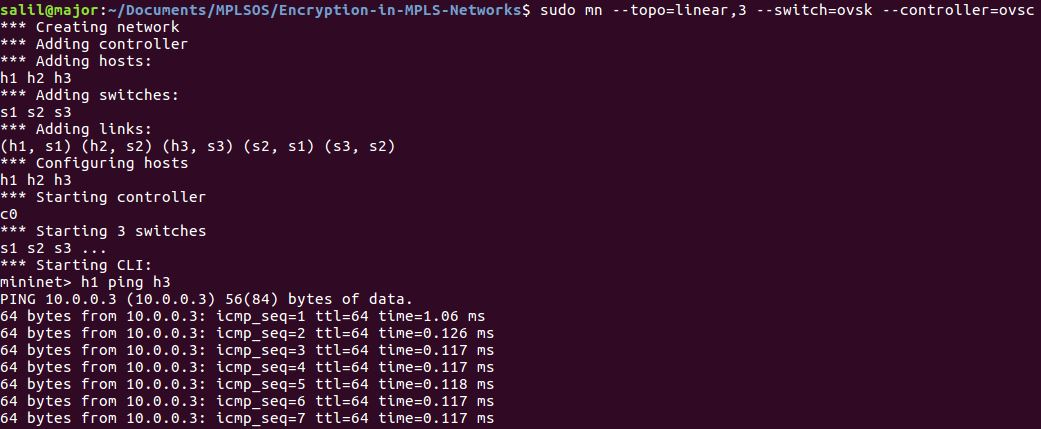
\includegraphics[width=\textwidth]{images/16_ICMP_responce_for_MPLS_OS.JPG}
   \caption{'ping' response for MPLS OS}
    \label{fig:compbest}
\end{figure}











